%%%%%%%%%%%%%%%%%%%%%%% file template.tex %%%%%%%%%%%%%%%%%%%%%%%%%
%
% This is a general template file for the LaTeX package SVJour3
% for Springer journals.          Springer Heidelberg 2010/09/16
%
% Copy it to a new file with a new name and use it as the basis
% for your article. Delete % signs as needed.
%
% This template includes a few options for different layouts and
% content for various journals. Please consult a previous issue of
% your journal as needed.
%
%%%%%%%%%%%%%%%%%%%%%%%%%%%%%%%%%%%%%%%%%%%%%%%%%%%%%%%%%%%%%%%%%%%
%
% First comes an example EPS file -- just ignore it and
% proceed on the \documentclass line
% your LaTeX will extract the file if required
\begin{filecontents*}{example.eps}
%!PS-Adobe-3.0 EPSF-3.0
%%BoundingBox: 19 19 221 221
%%CreationDate: Mon Sep 29 1997
%%Creator: programmed by hand (JK)
%%EndComments
gsave
newpath
  20 20 moveto
  20 220 lineto
  220 220 lineto
  220 20 lineto
closepath
2 setlinewidth
gsave
  .4 setgray fill
grestore
stroke
grestore
\end{filecontents*}
%
\RequirePackage{fix-cm}
%
%\documentclass{svjour3}                     % onecolumn (standard format)
%\documentclass[smallcondensed]{svjour3}     % onecolumn (ditto)
\documentclass[smallextended]{svjour3}       % onecolumn (second format)
%\documentclass[twocolumn]{svjour3}          % twocolumn
%
\smartqed  % flush right qed marks, e.g. at end of proof
%
\usepackage{graphicx}
%
% \usepackage{mathptmx}      % use Times fonts if available on your TeX system
%
% insert here the call for the packages your document requires
%\usepackage{latexsym}
% etc.
%
% please place your own definitions here and don't use \def but
% \newcommand{}{}
%
% Insert the name of "your journal" with
% \journalname{myjournal}
%
\begin{document}

\title{Not sure...:%\thanks{Grants or other notes
%about the article that should go on the front page should be
%placed here. General acknowledgments should be placed at the end of the article.}
}
\subtitle{Comparison of Twe women's mobility and associated traits at different reproductive stages}

%\titlerunning{Short form of title}        % if too long for running head

\author{Layne Vashro
}

%\authorrunning{Short form of author list} % if too long for running head

\institute{L. Vashro \at
              270 South 1400 East, Salt Lake City, UT 84112 \\
              Tel.: +001 (801) 581 6251\\
              \email{layne.vashro@anthro.utah.edu}           %  \\
}

\date{Received: date / Accepted: date}
% The correct dates will be entered by the editor


\maketitle

\begin{abstract}
Insert your abstract here. Include keywords, PACS and mathematical
subject classification numbers as needed.
\keywords{First keyword \and Second keyword \and More}
% \PACS{PACS code1 \and PACS code2 \and more}
% \subclass{MSC code1 \and MSC code2 \and more}
\end{abstract}

\section{Introduction}
\label{sec:1}
Researchers consistently find  that men perform better than women in certain spatial-cognitive and navigational tasks.  These differences are well-documented in Western industrialized societies and have increasingly been replicated cross-culturally (cite cite cite).  Evolutionary psychologists have put forward several distinct theories that link these sex differences to further differences in traveling long distances and into unfamiliar environments.  In most of these theories, past selection favored the males who could travel more safely and efficiently which required superior navigation ability and the spatial-cognitive traits that facilitate it \cite{gray1971sex}.  The key point of disagreement among these arguments is simply the presumed payoff of that travel (mates \cite{gaulin1992evolution}, hunting \cite{eals1994hunter}, or warfare \cite{geary1995sexual}).  However, one explanation for the sex differences in ranging, spatial cognition, and navigation ignores the payoffs to males and instead turns the focus on the fitness ramifications of women's long-distance mobility.  This ``fertility and parental care hypothesis'' put forward by \cite{sherry1997evolution} argues that the observed sex differences can be explained in terms of the potential costs to women traveling, particularly during key periods of reproduction.

	\subsection{Fertility and parental care}
	\label{sec:1.1}
The fertility and parental care hypothesis highlights the relationship between women's performance on spatial tasks and hormonal changes related to developmental and cyclical stages associated with reproduction.  In particular, the negative correlation between estrogen levels and spatial ability (Frye, 1994; Hampson and Kimura, 1988; Hausmann et al., 2000; Lacreuse et al. 2001; McCormick and Teillon, 2001; Warren and Juraska, 1997).  This relationship is interpreted as an adaptive mechanism for curtailing women's travel during reproductive periods in order to limit exposure to risks and the expenditure of excess calories.
	
Risky strategies tend to pay higher fitness dividends when variance in reproductive success among competitors is high (cite cite cite).  As is the case in many species, men's reproduction skews higher than women's (cite).  The constraints of women's extensive prepartum investment in offspring places a ceiling on potential reproduction, and in doing so limits the prospective bounty paid to risky strategies relative to men.  In addition to this common mammalian pattern, humans are a particularly altricial species.  Infants have an extended period of dependence, the burden of which falls predominantly on the mother in most societies.  Fitness calculations for men need to account for the potential loss of future offspring due to risky behavior, but at least in the subsistence societies that have been investigated, men's deaths do not endanger living children \cite{sear2008keeps}.  This is not the case for women, since the passing of a mother dramatically reduces any dependent children's likelihood of survival \cite{hill1996ache, sear2008keeps}.  The application of evolutionarily informed perspectives on risk has illuminated the discussion of sex-differences in violence, risky leisure activities, and even financial decision-making \cite{wilson1985competitiveness} \cite{wilson1997life} \cite{jianakoplos1998women}.

While less dramatic than some of the above examples, travel away from home is risky behavior.  Risks including large predators, snakes, inclement weather, exposure, falling rocks, and many other dangers are real concerns when navigating wild natural environments.  In many cases, interpersonal violence may also pose a serious cause for concern.  Finally, their is a non-zero risk of simply becoming lost and never finding home in a world without marked intersections, cellular phones, and GPS navigation systems (cite cite).  The nature of the risk has changed for many of us in today's world, but travel remains one of the riskier activities.  Travel related ``road injury'' is the seventh most common cause of death worldwide \cite{krug2000global}, and even in the United States traffic accidents are the second largest external cause of death \cite{sherry2010cdc}.  

In addition to the risks associated with travel, the fertility and parental care hypothesis also notes the energetic costs of traveling and how these trade-off against the need to divert as many calories as possible towards reproduction (cite).  With these concerns about the risks and energetic costs of travel in mind, the link between hormonal patterns associated with women's reproduction and the tools and desire to travel broadly presents an appealing evolutionary narrative.  However, the logical thread hangs on several assumptions about the relationship between demographics and life history and cognition and mobility that need to be demonstrated.

	\subsection{Predictions}
	\label{sec:1.2}
This paper sets out to test a series of predictions drawn from the fertility and parental care hypothesis.  In some cases this means replicating well-established patterns in a population that faces navigational challenges more similar to those faced by ancestral humans.  In other cases, we offer the first test of predictions that underpin the fertility and parental care hypothesis and/or help distinguish it from alternative evolutionary theories explaining human sex differences across these traits.	
	
\paragraph{1. Men will demonstrate higher spatial-cognitive and navigational ability, report lower spatial anxiety, and travel more broadly.}\mbox{}\\

Men tend to outperform women in spatial-cognitive that ask participants to mentally manipulate objects \cite{sanders1982sex} (Shepard and Metzler, 1971; Eals and Silverman, 1994; Lawton, 2010). Measures of navigational skill, especially those that tap into cues used in long-distance travel into unfamiliar environments also tend to favor men \cite{moffat1998navigation} (Bryant, 1982; Galea and Kimura, 1993; Henrie, Aron, Nelson, and Poole, 1997), though this difference is not as robust (Burke, Kandler, and Good, 2012; Evans, 1980; Gilmartin and Patton, 1984; Golledge, 1995; Montello, Richardson, Hegarty, and Provenza, 1999).  Women also report higher levels of spatial anxiety than men and are less confident in their navigational ability (Devlin and Bernstein, 1995; Kolakowski and Malina, 1974; Lawton and Kallai, 2002; Picucci, Caffo, and Bosco, 2011; Schmitz, 1997).  Finally, research across a remarkably broad spectrum of environmental and subsistence context has consistently found that men occupy larger ranges than women (Ecuyer-Dab and Robert, 2004b; Gaulin and Hoffman, 1988; MacDonald and Hewlett, 1999)

This collection of sex-differences captures the empirical pattern that led researchers to posit the fertility and parental care hypothesis, as well as the other competing hypotheses noted above.  Previous work among the Twe and Tjimba found that these groups do indeed conform to this expected sex-difference in spatial cognition, navigation, and ranging.  This study adds an improved measure of mental rotation and a measure of spatial anxiety.

\paragraph{2.  Women's spatial-cognitive and navigational ability will decline, spatial anxiety will increase, and range-sizes will shrink when women enter reproductive maturity, then all of these traits will revert after menopause}\mbox{}\\

According to the fertility and parental care hypothesis, sex differences in mobility and associated traits should emerge around puberty along with the constraints of reproduction.  Consistent with this expectation, sex differences in spatial ability first appear, or at least expand, near female reproductive maturity in several mammals including humans (rats, water maze: Kanit et al., 2000; rats, symmetrical maze: Krasnoff and Weston, 1976; humans, mainly pen and paper tests: Voyer et al., 1995).  Unlike most other mammals, humans also have an extended \emph{post}-reproductive period marked by decreased estrogen levels (cite cite).  Not only are women now freed from the constraints of rearing their own offspring, but this may actually be a time when mobility pays in allowing older women to travel to the homes of their daughters in order to assist in raising their grandchildren (blurton-jones).  This should be a time when women's mobility and associated traits increase, at least relative to their male counterparts.

\paragraph{3.  Reproductive-aged women's spatial-cognitive and navigational ability will decline, spatial anxiety will increase, and range-sizes will shrink when they are pregnant or lactating}\mbox{}\\

In addition to the simple distinction between pre/post reproductive women and reproductive-aged women, Jones et al. \cite{jones2003evolution} identify pregnancy and lactation as a specific period within a woman's reproductive career when minimizing risk and caloric expenditure may be particularly important...

%Female Gorillas (Gorilla gorilla gorilla) avoid transfers when they have infants \cite{watts1989infanticide, stokes2003female}.  Female Chimpanzees (Chimpanzee chimpanzee) typically disperse from their natal home when they reach reproductive maturity then never make a secondary transfer.  However, the threat of attacks from out-group males is a danger to females with dependent offspring travel the periphery of their home region. \cite{mitani2002recent, watts1989infanticide} (cite others also)

%Looking across the entire life-cycle, it is true that women's estrogen level rise as they enter reproductive maturity (is this tru?), and fall after menopause.  This lines up with the theory linking decreased mobility as a risk reduction strategy that is mediated by estrogen.  However, looking within women of reproductive age the pattern of estrogen cycles is more difficult to link with at least a simple version of risk reduction.  The problem is that women's estrogen level drop post-partum.  The team between  birth and weaning is likely \emph{the} time when the concerns highlighted by the fertility and parental care hypothesis should be most important. Instead, at least among mice, this period is associated with improved performance in maze tasks ans increased range (nest visits?... check this). 

\paragraph{4. Spatial cognition predicts women's range size.}\mbox{}\\

This prediction about the relationship between spatial ability and travel is uniquely useful in discriminating between the fertility and parental care hypothesis and the other evolutionary explanations that place the adaptive focus on male interests.  The argument that women's lower spatial ability is an adaptive mechanism to curtail risky ranging behavior necessarily assumes that women with lower spatial ability actually travel less.  Meanwhile, the alternative explanations necessarily assume a similar relationship between men's spatial ability and ranging behavior.  It is important to note that both the fertility and parental care hypothesis and the alternatives are agnostic to the relationship between cognition and ranging for the other sex, however, if we only see the relationship in one of the sexes it poses a challenge for any theory placing the other sex in an adaptive role.  Previous work among the Twe and Tjimba found a relationship between spatial cognition and ranging, but only among men.  However, the sample for that study was extremely small making Type II error a likely culprit.


\section{Methods}
\label{sec:2}
	\subsection{Population}
%This study includes all women living in the \emph{Ovizorowe} mountain valley in northwestern Namibia.  This sample includes mostly members of the Twe ethnic group who live in several villages dispersed throughout the valley, as well as women from some Himba and Tjimba communities bookending the valley. 

%While the Kunene region is remarkably ``wild'' and ``untouched'' by modern standards, it is likely much safer to travel than many ancestral environments.  Leopards and poisonous snakes are a legitimate concern, but most of the dangerous predators have been eliminated from the region due tot the threat they pose to cattle.  The threat of interpersonal and tribal violence is also much lower than in the not so distant past.  That said, participants did report concern about meeting strangers during travel and I encountered one small village in the mountains where a rapist had been targeting women when they visited their garden unaccompanied. 

		\subsubsection{Mental rotation}
		\label{sec:2.2.1}		
%The mental rotation task was based on the Mental Rotation Test (MRT) developed by \cite{shepard1971mental}. In the traditional task, objects created by configurations of cubes are presented to the viewer. These cubes are either rotated versions of the same cube or an entirely different cube. The viewer is then asked to decide if the cubes are the same or different. Both accuracy and response time are recorded. We designed an adapted computer-based version of the MRT using gaming software \cite{unity14} and conducted the experiment on a Toshiba 15.6" Touch-Screen laptop.  Due to the novel nature of rectilinear objects, for the Twe, we adapted the Mental Rotation Test by having the viewers make judgments about computer generated images of human bodies with one out stretched arm, which were rotated on a two-dimensional axis. Additionally, instead of showing the viewers two objects and asking them to make a same or different decision, we chose to show one target image at the top of the screen and have the viewer select one of two images that matched the target. This configuration was designed to avoid linguistic issues around having a button or icon that indicated same or different. Instead, the viewer simply used the touched screen interface to touch the body that matched the target object. 12 trials were presented to the viewers showing the bodies from the front and back, rotated twice at 0, 60, 120, 180, 240, and 300 degrees, making a total of 24 trials. This task was readily understood by most participants. However, it was unclear if some participants understood the task, as a few adopted a strategy where they only selected the left or right responses or alternated between the two. For this reason, only participants that scored above chance were used in the analyses. 

		\subsubsection{Real-world pointing}
		\label{sec:2.2.2}
%We used Real-world distant pointing accuracy as a measure of navigation abilities. Previous work has suggested that the ability to point to a location is a skill that is uniquely develop by mobility \cite{bell2004relationship}. In our task we selected XX locations that were designed to form a normal distribution of places that the Twe had likely visited with varying distances. We used a Brunton Pocket Transit International Compass with 0-360 Degree Scale mounted on a tripod to record the pointing data. Viewers were first asked if they had visited one of the locations. If they had, they were then asked to use the sight on the compass to point to the location. Degree measurements were then taken from the compass. Accuracy was measured by taking the GPS coordinates that the compass was located at and the coordinates of the location pointed to, then calculating the degree of error from were the viewer pointed and the actual location. This resulted in errors ranging from 0 degrees (perfectly accurate) to 180 degrees (completely in the wrong direction). Measurements were taken in locations that were free of objects that visually occluded participants’ views (e.g. dense foliage and mountains).

	\subsection{Mobility interviews}
	\label{sec:2.1}
%Participants were asked to name each place they traveled to and spent the night in the past year.  In addition, they were asked who they traveled with, who they stayed with, and why they made the trip.  These data were used to create two highly-correlated measures of annual range size.  1) The number of unique places visited in the past year, and 2) the number of kilometers needed to visit each place visited in the past year.  In addition, the analysis is able to discriminate between pair, group, and unaccompanied travel, and identify patterning in the function of travel.

\section{Results}
\label{sec:3}
	\subsection{Comparisons across demography and life history}
	\label{sec:3.1}
		\subsubsection{Spatial Cognition}		
		\label{sec:3.1.1}
		
According to predictions drawn from the fertility and parental care hypothesis, we should find that males perform better than women and women with unweaned infants perform worse than other reproductive-aged women.  We should also expect postmenopausal women to perform better than women still in the fertile stage of their career.

Men responded more accurately but slightly slower in the mental rotation task (see Table \ref{tab:cog}).  Postmenopausal women responded slower than reproductive-aged women and were slightly less accurate.  Actual expectations regarding the performance of postmenopausal women may be more complex than presented here, since there are likely confounding forces depressing performance of the older postmenopausal women.  However, comparing men split into analogous age groups the differences look similar but with a slightly weaker decline (Accuracy decrease from 89.6\% to 86.7\% and reaction time increase from 5.7 to 7.6).  It does not look like women's spatial ability improves after menopause even accounting for general age-based decline shared with men.  Breastfeeding women responded slightly quicker and more accurately to the mental rotation task than other women of reproductive age, but the differences are small enough to easily be explained by random chance.  The sample includes only three pregnant women, but two of them were among the eleven women to obtain a perfect score on the mental rotation task.

\begin{table}[h!]
\caption{Spatial Cognition}
\label{tab:cog}  
\begin{tabular}{lllllll}
\hline\noalign{\smallskip}
Comparison & \phantom{0}n$|$n & $\mu1$ & $\mu2$ & d & \multicolumn{2}{c}{95\% CI} \\
\noalign{\smallskip}\hline\noalign{\smallskip}
Men $|$ Women & 55$|$43 & 89.3\% & 82.7\% & \phantom{-}0.457* & \phantom{-}0.043 & \phantom{-}0.871 \\
& & 5.9 & 5.6 & \phantom{-}0.149 & -0.260 & \phantom{-}0.558 \\
Postmenopausal $|$ Not & \phantom{0}5$|$38 & 77.1\% & 83.4\% & -0.384 & -1.372 & \phantom{-}0.604 \\
& & 7.5 & 5.4 & \phantom{-}1.279* & \phantom{-}0.253 & \phantom{-}2.306 \\
Lactating $|$ Not & 21$|$14 & 83.7\% & 81.0\% & \phantom{-}0.163 & -0.561 & \phantom{-}0.888 \\
& & 5.4 & 5.8 & -0.276 & -1.002 & \phantom{-}0.450 \\
Pregnant $|$ Not & 3$|$14 & 92.6\% & 81.0\% & \phantom{-}0.803 & -0.678 & \phantom{-}2.285 \\
& & 3.7 & 5.8 & -1.760* & -3.377 & -0.143 \\
\noalign{\smallskip}\hline
\end{tabular}\par
\bigskip
d is Cohen's d measure of effect size \cite{cohen1988statistical}. First row under each group gives accuracy, and second row gives reaction times.  Comparisons where the 95\% confidence interval does not include 0 are denoted with a ``*''.
\end{table}		  

The patterning of participants dropped due to insufficient understanding complicates these findings.  The participants who were removed from the sample either due to failure in the practice or ultimately scoring below chance on the task were more likely to be women, specifically post-menopausal women.  Only 18.8\% of men who were shown the practice failed to demonstrate understanding compared to 28.3\% of the women.  Within the set of 64 women, 61.\% of the 16 post-menopausal participants failed to demonstrate understanding compared to 21.4\% of the younger women.  This limited understanding may be a function of some cognitive feature(s) unrelated to the spatial cognitive abilities in question, however, to whatever extent the traits of interest help explain their omission these results understate the difference between reproductive-aged and post-menopausal women's spatial cognition.


		\subsubsection{Navigation}
		\label{sec:3.1.2}

According to predictions drawn from the fertility and parental care hypothesis, we should find that males perform better than women and women with unweaned infants perform worse than other reproductive-aged women.  We should also expect postmenopausal women to perform better than women still in the fertile stage of their career.

\begin{table}[h!]
\caption{Navigation}
\label{tab:nav}  
\begin{tabular}{lllllll}
\hline\noalign{\smallskip}
Comparison & \phantom{0}n$|$n & $\mu1$ & $\mu2$ & d & \multicolumn{2}{c}{95\% CI} \\
\noalign{\smallskip}\hline\noalign{\smallskip}
Men $|$ Women & 61$|$57 & 15.18$^{\circ}$ & 19.22$^{\circ}$ & -0.481* & -0.855 & -0.108 \\
Postmenopausal $|$ Not & 14$|$43 & 20.54$^{\circ}$ & 18.79$^{\circ}$  & \phantom{-}0.188 & -0.441 & \phantom{-}0.816\\
Lactating $|$ Not & 24$|$17 & 16.73$^{\circ}$ & 20.97$^{\circ}$  & -0.422 & -1.087 & \phantom{-}0.243 \\
Pregnant $|$ Not & 3$|$17 & 24.98$^{\circ}$ & 20.97$^{\circ}$  & \phantom{-}0.330 & -1.342 & \phantom{-}2.002 \\
\noalign{\smallskip}\hline
\end{tabular}\par
\bigskip
Comparisons where the 95\% confidence interval does not include 0 are denoted with a ``*''.
\end{table}		  


Men outperformed women in the real-world pointing measure of navigational skill (see Table \ref{tab:nav}).  There do not appear to be any meaningful differences between postmenopausal and younger women in pointing accuracy.  Post-partum women performed considerably better than other reproductive-aged women, however, the 95\% confidence interval around the Cohen's D measure includes 0.  A larger sample may be needed to assess the relationship between navigation ability and both pregnancy and lactation.

% For one-column wide figures use
\begin{figure}[!htb]
  \includegraphics[width=0.75\textwidth]{QQ_3_Acc}
\caption{Please write your figure caption here}
\label{fig:1}       % Give a unique label
\end{figure}

		\subsubsection{Anxiety}
		\label{sec:3.1.2}
According to predictions drawn from the fertility and parental care hypothesis, we should find that males self-report lower spatial anxiety than women and women with unweaned infants report higher anxiety than other reproductive-aged women.  We should also expect postmenopausal women to report lower anxiety than women still in the fertile stage of their career.

\begin{table}[h!]
\caption{Spatial Anxiety}
\label{tab:anx}  
\begin{tabular}{lllllll}
\hline\noalign{\smallskip}
Comparison & \phantom{0}n$|$n & $\mu1$ & $\mu2$ & d & \multicolumn{2}{c}{95\% CI} \\
\noalign{\smallskip}\hline\noalign{\smallskip}
Men $|$ Women & 27$|$27 & 2.29 & 2.64 & -0.743* & -1.325 & -0.161 \\
Postmenopausal $|$ Not & \phantom{0}8$|$19 & 2.45 & 2.72  & -0.773 & -1.705 & \phantom{-}0.159\\
Lactating $|$ Not & 12$|$5 & 2.83 & 2.60 & \phantom{-}0.971 & -0.302 & \phantom{-}2.244 \\
Pregnant $|$ Not & 2$|$5 & 2.38 & 2.60 & -1.046 & -3.783 & \phantom{-}1.690 \\
\noalign{\smallskip}\hline
\end{tabular}\par
\bigskip
Comparisons where the 95\% confidence interval does not include 0 are denoted with a ``*''.
\end{table}		 


Consistent with expectations, men reported lower spatial anxiety than women (see Table \ref{tab:anx}).  The other comparisons also trend in the expected directions with postmenopausal women expressing lower spatial anxiety than younger women and postpartum women reporting more anxiety than their counterparts.  However, the samples for each of these latter comparison are very small, which allows the 95\% confidence interval around the Cohen's D to encompass 0 despite very strong effect sizes.

% For one-column wide figures use
\begin{figure}[!htb]
  \includegraphics[width=0.75\textwidth]{QQ_3_sax}
\caption{Please write your figure caption here}
\label{fig:1}       % Give a unique label
\end{figure}


		\subsubsection{Mobility}
		\label{sec:3.1.2}
Consistent with expectation, men are much more mobile than women.  Men had visited more than twice as many unique locations in the past year and those trips were almost twice as likely to be made without a companion (see Table \ref{tab:mob}).  Men also traveled slightly more than twice as far as women on a day-to-day basis around the home region.  

\begin{table}[h!]
\caption{Mobility}
\label{tab:mob}  
\begin{tabular}{lllllll}
\hline\noalign{\smallskip}
Comparison & \phantom{0}n$|$n & $\mu1$ & $\mu2$ & d & \multicolumn{2}{c}{95\% CI} \\
\noalign{\smallskip}\hline\noalign{\smallskip}
Men $|$ Women & 42$|$45 & 4.29 & 2.02 & \phantom{-}0.725* & \phantom{-}0.280 & \phantom{-}1.171 \\
& 40$|$40 & 46.4\% & 24.2\% & \phantom{-}0.586* & \phantom{-}0.125 & \phantom{-}1.046 \\
& 20$|$18 & 8.75km & 4.38km & \phantom{-}1.000* & \phantom{-}0.280 & \phantom{-}1.720 \\
Postmenopausal Not & 10$|$35 & 1.60 & 2.14 & -0.341 & -1.085 & \phantom{-}0.402 \\
& 10$|$30 & 35.0\% & 20.6\% & \phantom{-}0.390 & -0.374 & \phantom{-}1.154 \\
& \phantom{0}3$|$15 & 7.05km & 3.85km & \phantom{-}1.361 & -0.161 & \phantom{-}2.882 \\
Lactating $|$ Not & 20$|$12 & 2.80 & 1.33 & \phantom{-}0.899* & \phantom{-}0.091 & \phantom{-}1.707 \\
& 19$|$9 & 22.0\% & 22.2\%  & -0.008 & -0.872 & \phantom{-}0.855 \\
& 19$|$5 & 3.78km & 3.71km & \phantom{-}0.035 & -1.395 & \phantom{-}1.464 \\
Pregnant $|$ Not & 3$|$12 & 1 & 1.33 & -0.294 & -1.798 & \phantom{-}1.210 \\
& 2$|$9 & 0\% & 22.2\%  & -0.649 & -2.641 & \phantom{-}1.343\\
& 3$|$5 & 4.24km & 3.71km & \phantom{-}0.181 & -1.887 & \phantom{-}2.250 \\
\noalign{\smallskip}\hline
\end{tabular}\par
\bigskip
First row under each group gives accuracy, and second row gives reaction times.  Comparisons where the 95\% confidence interval does not include 0 are denoted with a ``*''.
\end{table}		

The fertility and parental care hypothesis predicts that postmenopausal women should be more mobile than women in the midst of their reproductive careers.  Postmenopausal Twe women actually reported visiting slightly fewer places in the past year (a decline that is nearly identical to that of similar-aged men), however, they did make a higher percentage of their trips unaccompanied which is consistent with the expectation of diminished risk-aversion.  This difference small enough that the 95\% confidence interval around the Cohen's D easily includes 0.  Among the three post-menopausal women to participate in the daily task, one recorded the highest average travel of all eighteen women included in the study (11.22 km), while the other two older women averaged a kilometer more daily travel than the average of the reproductive-aged women (4.97 km compared to 3.85 km).  A larger sample is clearly needed, but these initial findings are intriguing and consistent with expectation drawn from the fertility and parental care hypothesis.

% For one-column wide figures use
\begin{figure}[!htb]
  \includegraphics[width=0.75\textwidth]{QQ_3_tot}
\caption{Please write your figure caption here}
\label{fig:1}       % Give a unique label
\end{figure}


We expected pregnant and lactating women to curtail their mobility due to the risks and caloric costs of travel.  The three pregnant women had remained home most of the past year, and none of them made a single trip unaccompanied.  However, Twe women with unweaned children visited more than twice as many locations as other reproductive-aged women in the past year (see Figure \ref{fig:bfeed_tot}).  These visits were no more or less likely to be solo ventures.  There also does not appear to be any difference in daily travel. 		

	\subsection{Prediction 4: ... }
	\label{sec:3.1}
The fertility and parental care hypothesis predicts a positive relationship between spatial-cognitive ability and mobility. This expectation is shared with the other prominent theories linking spatial cognition to travel-based fitness effects, however, the others focus on this relationship in men rather than women.  Thus, looking at which sexes travel more in response to variance in spatial ability may help discriminate between possible explanations.	

\begin{table}[!tb]
\caption {Annual mobility and Spatial Cognition}
\label{tab:wm_spacemob}
  \centering
  \begin{tabular}{| l  ll  ll  ll  l |} 
    \hline   
  & \multicolumn{6}{c}{Independent Variables}& \\    
  & \multicolumn{2}{c}{MR} & \multicolumn{2}{c}{Male(1$|$0)} & \multicolumn{2}{c}{Male(1$|$0):MR} & $R^2$ \\
  & $Std. \beta$ & $Std. Err$ & $Std. \beta$ & $Std. Err$ & $Std. \beta$ & $Std. Err$  & \\
  Model 1 & 0.207\phantom{**} & 0.134\phantom{**} & & & & & 0.036\phantom{**} \\
  Model 2 & 0.262. & 0.137\phantom{**} & 0.331** & 0.114\phantom{**} & .300* & 0.131\phantom{**} & 0.222\\
  \hline 
  \end{tabular}  
{}
\end{table}

Mental rotation performance alone is only weakly predictive of travel in the past year and is not a statistically significant improvement over a null model ($M_{null} | M_1$, $\chi^2(1, 98) = 2.348, p = 0.121$).  However, including sex as an interaction effect dramatically improves model performance ($M_1 | M_2$, $\chi^2(2, 98) = 12.091, p = 0.0006$).  Interestingly, the direction of the effect is in the opposite direction of expectations drawn from the fertility and parental care hypothesis.  Men, but not women, with higher spatial ability appear to travel more broadly (see Figure \ref{fig:wm_acctot} and Table \ref{tab:wm_spacemob}).  This is consistent with findings in a previous study using a different measure of mental rotation (cite me).

% For one-column wide figures use
\begin{figure}[!htb]
  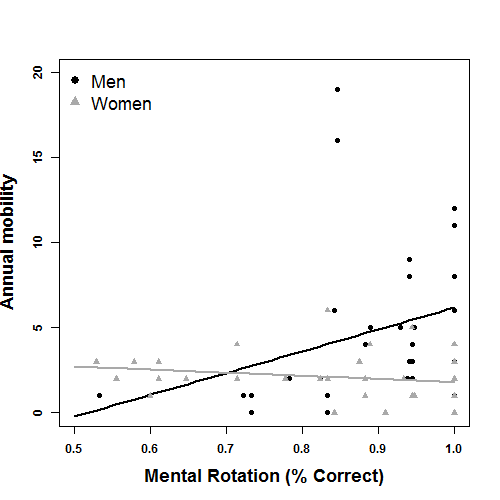
\includegraphics[width=0.75\textwidth]{mw_acctot}
\caption{Please write your figure caption here}
\label{fig:1}       % Give a unique label
\end{figure}

\section{Discussion}
\label{sec:4}

The observed sex differences across spatial cognition, navigation, spatial anxiety, annual mobility and daily mobility are all consistent with the fertility and parental care hypothesis.  Men outperformed women in the spatial-cognitive and navigational tasks, reported lower spatial anxiety, and traveled further at both scales.  However, all of these predictions apply equally well to the other prominent theories linking these traits in an evolutionary framework.  

The only area of this study that consistently fits expectations uniquely drawn from the fertility and parental care hypothesis is the spatial anxiety measure.  Postmenopausal women reported much lower anxiety than reproductive-aged women, and among the latter group, women currently dealing with an unweaned infant reported much higher anxiety.  Unfortunately, both of these tests lacked the power necessary to confidently reject random variance as an explanation for the patterning.  The mobility data also holds intriguing trends in the difference between postmenopausal and reproductive-aged women, with the older women moving much more on a daily basis and making a higher percentage of their annual visits abroad without accompaniment.  These trends are consistent with the fertility and parental care hypothesis but again lack statistical power.

Interestingly, one of the strongest findings of the study actually runs in the opposite direction of the fertility and parental care hypothesis.  Women with nursing infants traveled to more than twice as many unique locations as other reproductive-aged (and not pregnant) women in the past year.  The period between childbirth and the successful weaning of an infant is arguably the most vulnerable time in a woman's life in terms of travel risks.  Our measure of spatial anxiety shows women at this stage may appreciate things concerns. (does anxiety moderate??  I think it does)  However, these women actually expand on their annual travels in spite of this anxiety. 

......

%The additional 

%Scelza (cite) found that nearby Himba women travel more  

%One possible explanation for women's increased travel during the postpartum period is that they are trips   

%along these same lines.  Women with unweaned infants also performed better than other same-aged women in the real-world pointing measure of navigational ability.

%Comparing reproductive-aged women living in the \emph{Ovizorowe} Valley with and without nursing depends highlights interesting differences in both cognition and mobility.  Breastfeeding women performed better across our measures of spatial cognition (excepting the perspective-taking task), which is consistent with expectations based on the decline in estrogen associated with the post-partum period.  In addition, breastfeeding women were more mobile, traveling to more unique locations and covering more ground in doing so than their peers who were without an unweaned child over that period of time.  This increase in mobility may also be consistent with the down-tick in estrogen and improved spatial cognition from the perspective of several theories linking spatial cognitive ability to distant ranging.  

%These findings simultaneously support the patterns of cognition and behavior anticipated by the fertility and parental care hypothesis while complicating the interpretation with the fact that women are most mobile exactly when it seems least likely from the perspective of minimizing risk to offspring.

%Why would it be beneficial for women to range further when they have unweaned children?  One study among conducted among a nearby  Himba population (Scelza) showed women traveling the most to visit their mothers during periods of peak childcare need.  This seems an appealing answer to this situation as well, however, most of these women were actually moving \emph{away} from their mothers (is this true??) as a much greater fraction of this population lives matrilocally.  In addition, none of the women explicitly cited visiting their mother.  Several other alternatives... 1) ``Facebook'' effect...  ``Look at the baby, look at the baby''... making connections to relatives who may be called on in future times of need.  2) Rape deterred... then what about pregnancy??  Don't like this.

%Interested in future work looking at the volume and function of women's postpartum mobility in other populations, including the US.


%\begin{acknowledgements}
%If you'd like to thank anyone, place your comments here
%and remove the percent signs.
%\end{acknowledgements}

% BibTeX users please use one of
%\bibliographystyle{spbasic}      % basic style, author-year citations
%\bibliographystyle{spmpsci}      % mathematics and physical sciences
%\bibliographystyle{spphys}       % APS-like style for physics
%\bibliography{}   % name your BibTeX data base

% Non-BibTeX users please use
\bibliography{bfeed_refs}
\bibliographystyle{spbasic}      % basic style, author-year citations

\end{document}
% end of file template.tex
